\documentclass[a4paper]{scrreprt}
\usepackage{fullpage} % Slightly more margins
\usepackage{amsfonts}
\usepackage{fancyhdr}
\pagestyle{fancy}
\usepackage[english]{babel}
\selectlanguage{english}
\usepackage[utf8]{inputenc}
\usepackage{graphicx}
\usepackage{url}
\usepackage{textcomp}
\usepackage{amsmath}
\usepackage{lastpage}
\usepackage{pgf}
\usepackage{wrapfig}
\usepackage{fancyvrb}
\usepackage{listings} % Source code highlighting
\usepackage{algpseudocode} % Algorithms
\usepackage{courier}

% Create header and footer
\headheight 27pt
\pagestyle{fancyplain}
\lhead{\footnotesize{Object-Oriented Design, IV1350}}
\chead{}
\rhead{\footnotesize{Assignment 3 Report}}
\lfoot{}
\cfoot{\thepage (\pageref{LastPage})}

% Create title page
\title{Assignment 3}
\subtitle{Object-Oriented Design, IV1350}
\author{Emil Tullstedt emiltu@kth.se}
\date{2014-04-29}

\graphicspath{ {./images/} }
\lstset{basicstyle=\footnotesize\ttfamily, language=Java, numbers=left}

\begin{document}

\maketitle

\tableofcontents %Generates the TOC

\chapter{Introduction}
This report describes the implementation of a previously designed cache simulator made for a pregraduate project in the course \textbf{IV1350} at KTH in Stockholm. The implementation is not for production usage.

\begin{small}
While implementing the application, I co-operated with \textit{Martin Alge}, \textit{Jesper Falk} and \textit{Erik Pettersson}.
\end{small}

\chapter{Method}
In the process of procuring a working application that would run an implementation of the design bescribed in \textit{Assignment 2}\footnote{http://web.ict.kth.se/$\sim$emiltu/iv1350-emiltu-s2.pdf} Java were selected as being the preferred language in the documentation of the course.

The Java environment during the course of developing the application have consisted of the following:

\begin{itemize}
	\item OpenJDK Runtime Environment (\textbf{IcedTea} 2.4.4) (7u51-2.4.4-0ubuntu0.13.10.1)
	\item \textbf{rake} 10.3.0
	\item \textbf{rakejava} 1.3.7
	\item \textbf{javac} 1.7.0\_51
	\item \textbf{git} 1.8.3.2
\end{itemize}

As the application was already largely designed, implementation was made simplified. As the design was having a largely low coupling - it was possible to implement the separate classes for the design one by one, thus rapidly having a working application. The application were mostly written after the design with modifications were seemingly proper. During a period in the development process, the classes \texttt{CacheLayout} and \texttt{AddressLayout} was merged in the \texttt{CacheLayout}-class, but that idea was quickly scrapped since the class were dangerously close to becoming a megamodel containing most of the logic in the application.

The tests made their way into the application quite late, which have caused a couple of hours of unnecessary debugging for bugs that would've been quickly discovered if the tests had been written before the actual code of the application, as the bugs were mostly quite a proof of my errors.

\chapter{Result}
\label{sec:result}

\begin{figure}[h]
  \begin{center}
    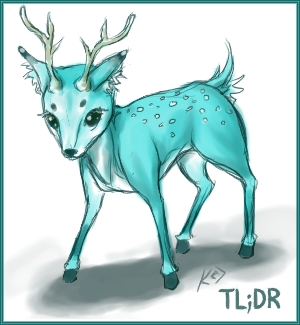
\includegraphics[scale=.5]{tldr.jpg}
    \caption{Teal Deer}
    \label{fig:sd}
  \end{center}
\end{figure}

\section{View, Controller and Startup}
\label{sec:sup}

In order to launch the application, there is need for a class handling the initialization of the controller and the view (which isn't fully covered in this report) and containing a \texttt{public static void main(String[] args)} function to be able to run the application from command-line. The class containing main is available in the \texttt{CacheSimulator}-class which source-code is available in subsection \ref{subsec:cachesimulator.java}.

The \texttt{CacheSimulator}-class initializes an object of the class \texttt{Controller} (which source is in subsection \ref{subsec:controller.java}) which handles the communication between the model classes and the \texttt{View}.


\subsection{Class: CacheSimulator}
\label{subsec:cachesimulator.java}
\lstinputlisting[language=Java]{cachesim/source/is/mjuk/cache/CacheSimulator.java}

\subsection{Class: Controller}
\label{subsec:controller.java}
\lstinputlisting[language=Java]{cachesim/source/is/mjuk/cache/Controller.java}

\subsection{Class: View}
\label{subsec:view.java}
\lstinputlisting[language=Java]{cachesim/source/is/mjuk/cache/View.java}

\subsection{Class: Storage}
\label{subsec:storage.java}
\lstinputlisting[language=Java]{cachesim/source/is/mjuk/cache/Storage.java}

\subsection{Class: SimulationDTO}
\label{subsec:simulationdto.java}
\lstinputlisting[language=Java]{cachesim/source/is/mjuk/cache/SimulationDTO.java}

\section{User}
\label{sec:user}

\subsection{Class: User}
\label{subsec:user.java}
\lstinputlisting[language=Java]{cachesim/source/is/mjuk/cache/User.java}

\section{Cache- and AddressLayout}
\label{sec:cache}

The CacheLayout is created by the controller when the user have required for it's creation.

\begin{algorithmic}
\State $x \in \mathbb{R} \geq 0$ 
\If {$i \in 2^x$}
    \State $\text{size of address element} \gets \log _2 i$ 
\EndIf
\end{algorithmic}

\subsection{Class: CacheLayout}
\label{subsec:cachelayout.java}
\lstinputlisting[language=Java]{cachesim/source/is/mjuk/cache/CacheLayout.java}

\subsection{Class: LayoutDTO}
\label{subsec:layoutdto.java}
\lstinputlisting[language=Java]{cachesim/source/is/mjuk/cache/LayoutDTO.java}

\subsection{Class: AddressDTO}
\label{subsec:addressdto.java}
\lstinputlisting[language=Java]{cachesim/source/is/mjuk/cache/AddressDTO.java}

\section{Instructions}

\subsection{Enum: InstructionType}
\label{subsec:instructiontype.java}
\lstinputlisting[language=Java]{cachesim/source/is/mjuk/cache/InstructionType.java}

\subsection{Class: Instruction}
\label{subsec:instruction.java}
\lstinputlisting[language=Java]{cachesim/source/is/mjuk/cache/Instruction.java}

\subsection{Class: InstructionDTO}
\label{subsec:instructiondto.java}
\lstinputlisting[language=Java]{cachesim/source/is/mjuk/cache/InstructionDTO.java}

\subsection{Class: DataCache}
\label{subsec:datacache.java}
\lstinputlisting[language=Java]{cachesim/source/is/mjuk/cache/DataCache.java}

\subsection{Class: Block}
\label{subsec:block.java}
\lstinputlisting[language=Java]{cachesim/source/is/mjuk/cache/Block.java}

\section{Tests}

\subsection{Class: CacheLayout Test}
\label{subsec:cachelayouttest.java}
\lstinputlisting[language=Java]{cachesim/test/is/mjuk/cache/CacheLayoutTest.java}

\subsection{Class: DataCache Test}
\label{subsec:cachelayouttest.java}
\lstinputlisting[language=Java]{cachesim/test/is/mjuk/cache/DataCacheTest.java}

\subsection{Class: Storage Test}
\label{subsec:cachelayouttest.java}
\lstinputlisting[language=Java]{cachesim/test/is/mjuk/cache/StorageTest.java}

\chapter{Discussion}

\chapter{Attachements}

\subsection{Class: MisMath}
\label{subsec:mismath.java}
\lstinputlisting[language=Java]{cachesim/source/is/mjuk/utils/MisMath.java}

\end{document}
